\documentclass[a4paper,12pt]{article}
\usepackage[a4paper, margin=2.5cm]{geometry}
\usepackage[pdftex]{graphicx}
\usepackage{tikz}
\usepackage{pgfplots}
\usepackage{enumitem}
\usepackage{float}
\usepackage[document]{ragged2e}
\usepackage[utf8]{inputenc}
\usepackage[T1]{fontenc}
\usepackage[spanish,es-tabla]{babel}
\renewcommand{\shorthandsspanish}{}
\usepackage{xurl}
\usepackage{lipsum}
\usepackage{mwe}
\usepackage{multicol}
\usepackage{siunitx}
\usepackage{listings}
\usepackage{circuitikz}

\graphicspath{ {/home/saikkopat/Documents/school/CE/P2/figures/} }

\title{Práctica 2: Ley de Ohm}
\author{González Cárdenas Ángel Aquilez \and Sánchez González Daniel Iván}

\begin{document}

\begin{titlepage}
	\begin{tikzpicture}[overlay, remember picture]
		\path (current page.north east) ++(-0.3,-1.5) node[below left] {
\includegraphics[width=0.35\textwidth]{/home/saikkopat/Documents/LOGOS IPN/EscudoESCOM}};
	\end{tikzpicture}
	\begin{tikzpicture}[overlay, remember picture]
		\path (current page.north west) ++(1.5,-1) node[below right] {
\includegraphics[width=0.2\textwidth]{/home/saikkopat/Documents/LOGOS IPN/logo}};
	\end{tikzpicture}
	\begin{center}
		\vspace{-1.5cm}
		{\LARGE Instituto Politécnico Nacional\par}
		\vspace{.5cm}
		{\LARGE Escuela Superior de Cómputo\par}
		\vspace{.5cm}
		{\Large Laboratorio de Circuitos Eléctricos\par}
		\vspace{2cm}
		{\large Unidad de aprendizaje:}\\{\Large Circuitos Eléctricos\par}
		\vspace{2cm}
		{\scshape\Huge Práctica 2\par}
		{\itshape\Large Ley de Ohm\par}
		\vfill
		\vspace{.7cm}
		{\Large Grupo: 3CV2\par}
		\vspace{.7cm}
		{\Large Integrantes:\\González Cárdenas Ángel Aquilez\\Sánchez González Daniel Iván\par}
		\vspace{1cm}
		{\Large Profesor: Vázquez Ortíz Mijaíl\par}
		\vspace{1cm}
		{\large Fecha de realización: 13 de marzo de 2023\par}
		{\large Fecha de entrega: 21 de marzo de 2023\par}
		\vfill
	\end{center}
\end{titlepage} 

\newpage

\tableofcontents

\newpage

\usepgfplotslibrary{units}

\section*{Objetivo}

\textbf{Objetivo}: El alumno comprenderá y manejará la adecuada interpretación de la Ley de Ohm, para que al finalizar la práctica este en posibilidades de:\par

\begin{itemize}
	\item Calcular los voltajes, corrientes y resistencias que están presentes en un circuito.
	\item Comprender el comportamiento de la corriente con respecto al voltaje y con respecto a la resistencia.
	\item Deducir la Ley de Ohm.
\end{itemize}


El alumno utilizara los siguientes materiales y equipo:

\begin{multicols}{2}
\textbf{Equipo}\\
\begin{itemize}[nosep]
	\item 1 Multímetro digital
	\item 1 Fuente de voltaje variable
\end{itemize}

\columnbreak

\textbf{Material}\\
\begin{itemize}[nosep]
	\item 1 \textit{Protoboard}
	\item 1 Resistor de \SI{1}{\kohm} a $\frac{1}{4}$ de \si{\watt}
	\item 1 Resistor de \SI{1}{\ohm} a \SI{1}{\W}
	\item 1 Potenciómetro de \SI{2.5}{\kohm} o mayor
	\item 4 puntas banana-caimán
	\item 2 puntas caimán-caimán
	\item Alambres para conexiones
\end{itemize}

\end{multicols}

\section{Desarrollo}

\subsection{Dependencia del voltaje}

Sin encender la fuente de voltaje, se fijó el valor del potenciómetro a \SI{2.5}{\kohm} y se armó el circuito de la Figura 1 sobre el \textit{protoboard}. Después de encendió la fuente de voltaje y se aumentó el valor suministrado de \SI{0}{\volt} hasta \SI{15}{\volt}, generando los resultados de la Tabla 1.

\vspace{0.5cm}

\begin{figure}[h!]
	\centering
	  \begin{circuitikz}[american, voltage dir=RP] 
	  		\draw	(0,0) 
	  		to[battery, name=E, v=$E$] (0,5)
	  		to[rmeterwa, t=A, v=$ $] (3,5)
	  		to[pR, l=Potenciómetro] (3,2.5)
			to[R, a=$R$, l=$\SI{1}{\kohm}$] (3,0) -- (0,0);
			\ctikztunablearrow{1}{1.5}{-30}{E}
		\end{circuitikz}
	\caption{Circuito 1}
\end{figure}

\vspace{1cm}

\begin{table}[ht!]
\begin{center}
\begin{tabular}{|c c c|}
	\hline
		Fuente de voltaje & Medición de la corriente & Calculo del valor de la corriente\\ [0.5ex]
	\hline
	\SI{0}{\volt} & \SI{-1.5}{\uA} & \SI{0}{\A} \\ \hline
	\SI{1}{\volt} & \SI{167}{\uA} & \SI{280}{\uA} \\ \hline
	\SI{2}{\volt} & \SI{335}{\uA} & \SI{570}{\uA} \\ \hline
	\SI{3}{\volt} & \SI{504}{\uA} & \SI{850}{\uA} \\ \hline
	\SI{4}{\volt} & \SI{672}{\uA} & \SI{1.1}{\mA} \\ \hline
	\SI{5}{\volt} & \SI{840}{\uA} & \SI{1.4}{\mA} \\ \hline
	\SI{6}{\volt} & \SI{1.008}{\mA} & \SI{1.7}{\mA} \\ \hline
	\SI{7}{\volt} & \SI{1.175}{\mA} & \SI{2}{\mA} \\ \hline
	\SI{8}{\volt} & \SI{1.343}{\mA} & \SI{2.2}{\mA} \\ \hline
	\SI{9}{\volt} & \SI{1.511}{\mA} & \SI{2.5}{\mA} \\ \hline
	\SI{10}{\volt} & \SI{1.678}{\mA} & \SI{2.8}{\mA} \\ \hline
	\SI{11}{\volt} & \SI{1.840}{\mA} & \SI{3.1}{\mA} \\ \hline
	\SI{12}{\volt} & \SI{2.013}{\mA} & \SI{3.4}{\mA} \\ \hline
	\SI{13}{\volt} & \SI{2.182}{\mA} & \SI{3.7}{\mA} \\ \hline
	\SI{14}{\volt} & \SI{2.350}{\mA} & \SI{4}{\mA} \\ \hline
	\SI{15}{\volt} & \SI{2.517}{\mA} & \SI{4.2}{\mA} \\ \hline
\end{tabular}
\label{table:1}
\caption{Mediciones de corriente con voltaje variable}
\end{center}
\end{table}

\vspace{1cm}

De la Tabla 1, se trazo la siguiente gráfica que contrasta los valores de corriente medidos y los valores calculados:

\vspace{1cm}

\begin{figure}[h!]
	\centering
	
\begin{tikzpicture}

\begin{axis} [change y base,
	y SI prefix=milli,
	legend style={legend pos=outer north east},
	width=12cm,	
	grid=both,
	ymin=0,
	xmin=0, xmax=15,
	xtick={0,...,15},
	title=Dependencia del voltaje,
	ylabel=Corriente (en \si{\mA}),
	xlabel=Voltaje,
]

\addplot [color=blue] coordinates {
			(0, 0)
			(1, 0.000167)
			(2, 0.000335)
			(3, 0.000504)
			(4, 0.000672)
			(5, 0.000840)
			(6, 0.001008)
			(7, 0.001175)
			(8, 0.001343)
			(9, 0.001511)
			(10, 0.001678)
			(11, 0.001840)
			(12, 0.002013)
			(13, 0.002182)
			(14, 0.002350)
			(15, 0.002517)
};
\addlegendentry{Mediciones}

\addplot [
	color=red,
	domain = 0:15,
	samples = 15,
] {x/3500};
\addlegendentry{Cálculos}

\end{axis}
\end{tikzpicture}

\end{figure}


\subsection{Dependencia de la resistencia}

Con la fuente de voltaje apagada, se fijó el valor del potenciómetro a \SI{0}{\ohm}. Se armó el circuito que se ilustra en la Figura 2 sobre el \textit{protoboard}. Después, se encendió la fuente de voltaje y se suministraron \SI{15}{\volt} para después variar el valor del potenciómetro según la Tabla 2:

\vspace{0.5cm}

\begin{figure}[h!]
	\centering
	  \begin{circuitikz}[american, voltage dir=RP] 
	  		\draw	(0,0) 
	  		to[battery, name=E, v=$E$] (0,5)
	  		to[rmeterwa, t=A, v=$ $] (3,5)
	  		to[pR] (3,2.5)
			to[R, a=$R$, l=$\SI{1}{\kohm}$] (3,0) -- (0,0);
			\draw (5,5) -- (5.5,5)
			to[rmeterwa, t=\si{\ohm}] (5.5,0) -- (5,0);
			\ctikztunablearrow{1}{1.5}{-30}{E}
		\end{circuitikz}
	\caption{Circuito 2}
\end{figure}

\vspace{1cm}

\begin{table}[ht!]
\begin{center}
\begin{tabular}{|c c c c|}
	\hline
		Valor del potenciómetro & Resistencia total & Corriente medida & Corriente calculada\\ [0.5ex]
	\hline
	\SI{0}{\ohm} & \SI{1}{\kohm} & \SI{15.156}{\mA} & \SI{15}{\mA}\\ \hline
	\SI{250}{\ohm} & \SI{1.25}{\kohm} & \SI{13.246}{\mA} & \SI{12}{\mA}\\ \hline
	\SI{500}{\ohm} & \SI{1.5}{\kohm} & \SI{11.100}{\mA} & \SI{10}{\mA}\\ \hline
	\SI{750}{\ohm} & \SI{1.75}{\kohm} & \SI{8.857}{\mA} & \SI{8.5}{\mA}\\ \hline
	\SI{1000}{\ohm} & \SI{2}{\kohm} & \SI{7.490}{\mA} & \SI{7.5}{\mA}\\ \hline
	\SI{1250}{\ohm} & \SI{2.25}{\kohm} & \SI{6.620}{\mA} & \SI{6.6}{\mA}\\ \hline
	\SI{1500}{\ohm} & \SI{2.5}{\kohm} & \SI{6.083}{\mA} & \SI{6}{\mA}\\ \hline
	\SI{1750}{\ohm} & \SI{2.75}{\kohm} & \SI{5.334}{\mA} & \SI{5.4}{\mA}\\ \hline
	\SI{2000}{\ohm} & \SI{3}{\kohm} & \SI{4.990}{\mA} & \SI{5}{\mA}\\ \hline
	\SI{2250}{\ohm} & \SI{3.25}{\kohm} & \SI{4.654}{\mA} & \SI{4.6}{\mA}\\ \hline
	\SI{2500}{\ohm} & \SI{3.5}{\kohm} & \SI{4.106}{\mA} & \SI{4.2}{\mA}\\ \hline
\end{tabular}
\label{table:2}
\caption{Mediciones de corriente con resistencia variable}
\end{center}
\end{table}

\vspace{1cm}

De manera similar, la siguiente gráfica contrasta los valores ideales contra las mediciones realizadas:

\vspace{1cm}

\begin{figure}[h!]
	\centering
	
\begin{tikzpicture}

\begin{axis} [change x base,change y base,
	x SI prefix=kilo,
	y SI prefix=milli,
	legend style={legend pos=outer north east},
	width=13cm,
	grid=both,
	ymin=0.0040, ymax=0.016,
	xmin=1000, xmax=3500,	xtick={1000,1250,1500,1750,2000,2250,2500,2750,3000,3250,3500},
	title=Dependencia de la resistencia,
	ylabel=Corriente (en \si{\mA}),
	xlabel=Resistencia (en \si{\kohm}),
]

\addplot [color=blue] coordinates {
			(1000, 0.015156)
			(1250, 0.013246)
			(1500, 0.011100)
			(1750, 0.008857)
			(2000, 0.007498)
			(2250, 0.006620)
			(2500, 0.006083)
			(2750, 0.005334)
			(3000, 0.004990)
			(3250, 0.004654)
			(3500, 0.004106)
};
\addlegendentry{Mediciones}

\addplot [
	color=red,
	domain = 1000:3500,
	samples = 11,
] {15/x};
\addlegendentry{Cálculos}

\end{axis}
\end{tikzpicture}

\end{figure}



\subsection{Potencia en los resistores}

Sin utilizar el \textit{protoboard} se armó el circuito que se ilustra en la Figura 3, donde se utilizó la resistencia de \SI{1}{\kohm} a $\frac{1}{4}$ \si{\watt} y se alimentó el circuito con \SI{1}{\volt}.

\vspace{0.5cm}

\begin{figure}[h!]
	\centering
	  \begin{circuitikz}[american, voltage dir=RP] 
	  		\draw	(0,0) 
	  		to[battery, v=$\SI{1}{\volt}$] (0,4)
	  		to[rmeterwa, t=A, v=$ $] (3,4)
			to[R, a=$R$, l=$\SI{1}{\kohm}$] (3,0) -- (0,0);
		\end{circuitikz}
	\caption{Circuito 3}
\end{figure}

\vspace{1cm}

Así, se logró dar respuesta a las siguientes preguntas planteadas durante la realización de la práctica:\par

\begin{itemize}
	\item ¿Cuál es el valor de la corriente? $i = \SI{0.829}{\mA}$.
	\item ¿Cuál es el valor de la potencia que disipa la resistencia? Como $P_R = i \times \si{\volt} = (\SI{0.829}{\mA})(\SI{1}{\volt}) = \SI{0.829}{\mW}$.
	\item ¿Qué efecto sucedió en la resistencia? Ninguno, pues la corriente máxima que soporta el resistor es de \SI{250}{\mA} y la corriente que circula en el circuito es de \SI{0.829}{\mA}.
\end{itemize}

\vspace{1cm}

Por último, del circuito anterior, se reemplazó el resistor con el resistor de \SI{1}{\ohm} a $\frac{1}{4}$\si{\watt}, como se ilustra en en la Figura 4:

\vspace{0.5cm}

\begin{figure}[h!]
	\centering
	  \begin{circuitikz}[american, voltage dir=RP] 
	  		\draw	(0,0) 
	  		to[battery, v=$\SI{1}{\volt}$] (0,4)
	  		to[rmeterwa, t=A, v=$ $] (3,4)
			to[R, a=$R$, l=$\SI{1}{\ohm}$] (3,0) -- (0,0);
		\end{circuitikz}
	\caption{Circuito 4}
\end{figure}

\vspace{1cm}

De manera similar, se contestan las siguientes preguntas planteadas durante la realización de la práctica:\par

\begin{itemize}
	\item ¿Cuál es el valor de la corriente? $i = \SI{0.910}{\A}$.
	\item ¿Cuál es el valor de la potencia que disipa la resistencia? Como $P_R = i \times \si{\volt} = (\SI{0.910}{\A})(\SI{1}{\volt}) = \SI{0.910}{\W}$.
	\item ¿Qué efecto sucedió en la resistencia? Se calentó la resistencia.
	\item ¿Cuál es la diferencia con el circuito anterior? El valor de la corriente y la potencia disipada.
	\item ¿Por qué? Como la resistencia es mejor, la corriente incrementa, entonces, la potencia que disipa el resistor es mayor; al no alcanzar su límite máximo, se calienta pero no se incendia.
\end{itemize}

\newpage

\section{Conclusiones}

\vspace{.5cm}

{\Large González Cárdenas Ángel Aquilez}\\
\vspace{.3cm}
Después de la realización de la práctica se logró apreciar la relación que establece la Ley de Ohm, pues en la primer parte, al aumentar el voltaje en circuito donde su resistencia no varia, la corriente aumenta; después, en la segunda parte, al tener un voltaje constante y una resistencia cuyo valor aumenta, la corriente disminuye. Finalmente, en la tercera parte, se apreció el efecto que la potencia produce de manera tangible en los elementos resistivos, al calentar el resistor de \SI{1}{\ohm} con una corriente cercana a \SI{1}{\A}.\par

\vspace{1cm}

{\Large Sánchez González Daniel Iván}\\
\vspace{.3cm}

Se concluye así la dependencia de la corriente con respecto al voltaje y la resistencia presentes en un circuito. También se logró apreciar el impacto que tiene la tolerancia de los elementos resistivos en la corriente de un circuito, ya que para el Circuito 1, la corriente fue de menor intensidad producto del valor de la resistencia total presente en el circuito. Finalmente, se utilizaron los valores de corriente y voltaje para determinar la potencia disipada por los elementos resistivos y se omitió el uso del valor resistivo debido a la tolerancia presente en ambos resistores que generan inconsistencia en los cálculos realizados con las mediciones.\par

\section{Anexos}
\subsection{Simulaciones de los circuitos}

A continuación de presentan los resultados de las simulaciones de los circuitos de las figuras 1, 2, 3 y 4 para contrastarlos con las mediciones y cálculos realizados. Se generaron gracias a la aplicación multiplataforma \textit{EveryCircuit}\texttrademark. \\

\vspace{.5cm}

\begin{figure}[!h]
\centering
	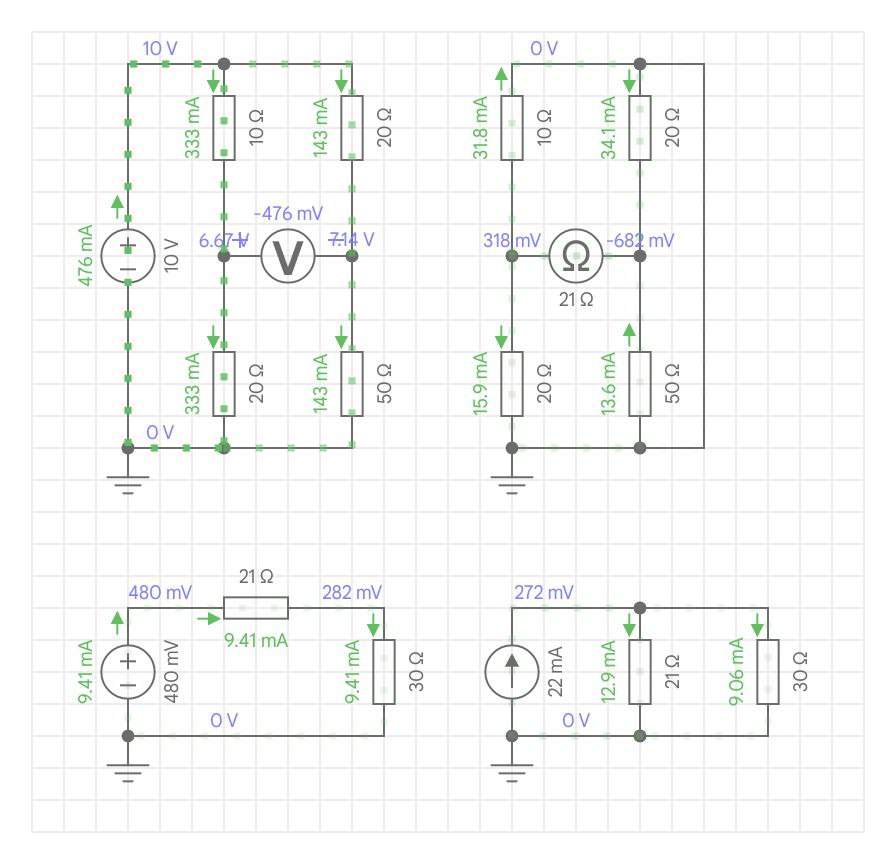
\includegraphics[width=.7\textwidth]{fig1}
	\label{fig5}
	 \caption{Simulación del Circuito 1}
\end{figure}


\vspace{.5cm}

\begin{figure}[!h]
\centering
	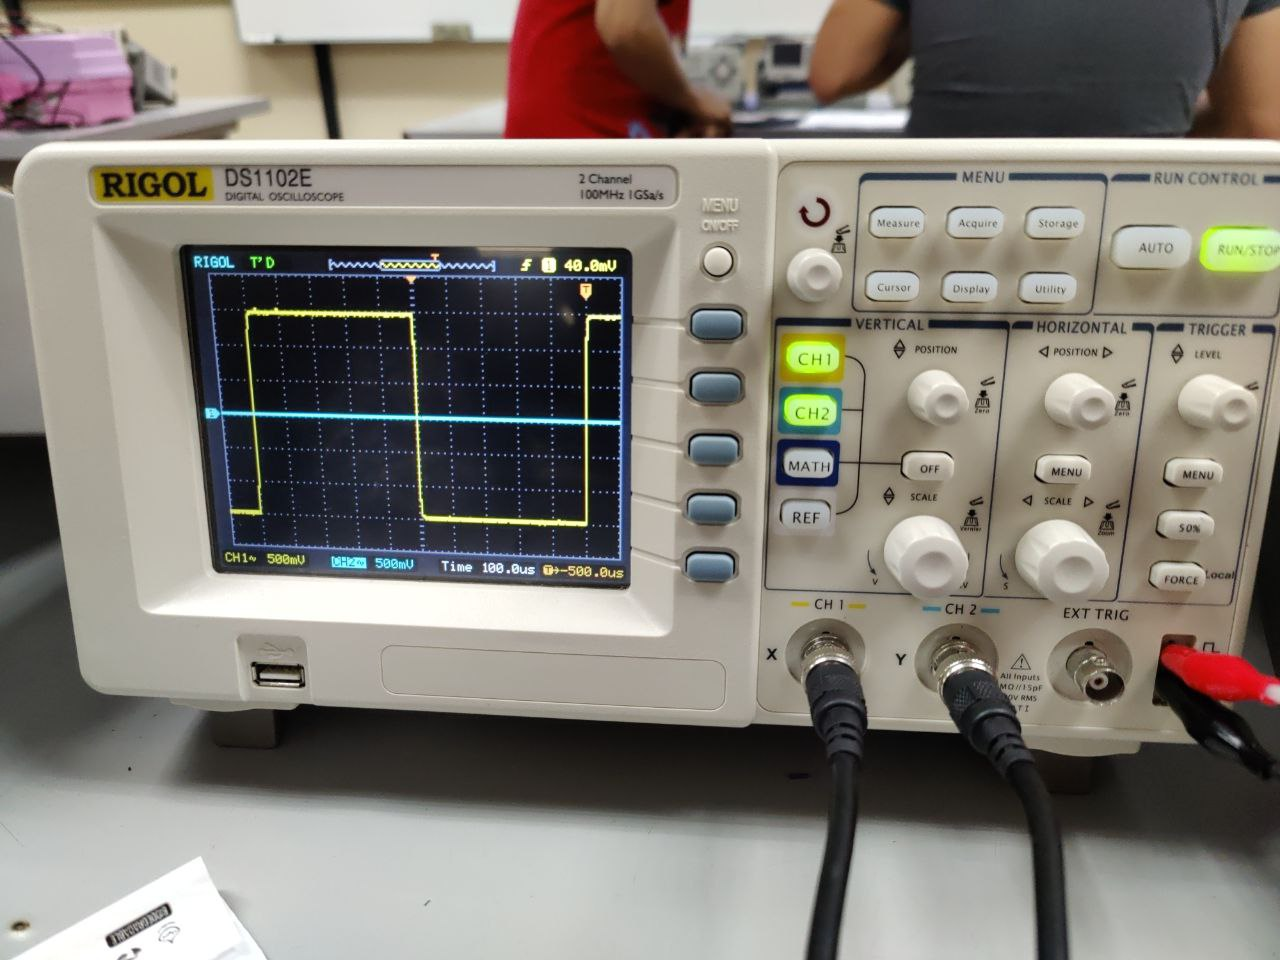
\includegraphics[width=.7\textwidth]{fig2}
	\label{fig5}
	 \caption{Simulación del Circuito 2}
\end{figure}

\vspace{.5cm}


\begin{figure}[!h]
\centering
	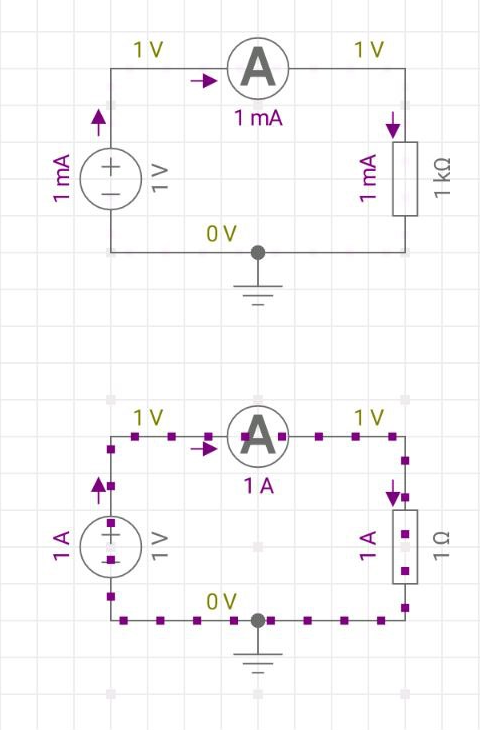
\includegraphics[width=.5\textwidth]{fig3}
	\label{fig5}
	 \caption{Simulaciones de los circuitos 3 y 4}
\end{figure}

\vspace{.5cm}

\end{document}